% Latex Header
\documentclass[12pt]{article}
\textwidth 16.5cm \oddsidemargin 0cm \topmargin -2cm \textheight
24cm \footskip 0.5cm
\usepackage{graphicx,pdfpages,caption,subcaption,amsmath,gensymb, minted, booktabs}
\usepackage[export]{adjustbox}[2011/08/13]
\def\n{\noindent}
\def\u{\underline}
\def\hs{\hspace}

\begin{document}

%% Cover Sheet %%
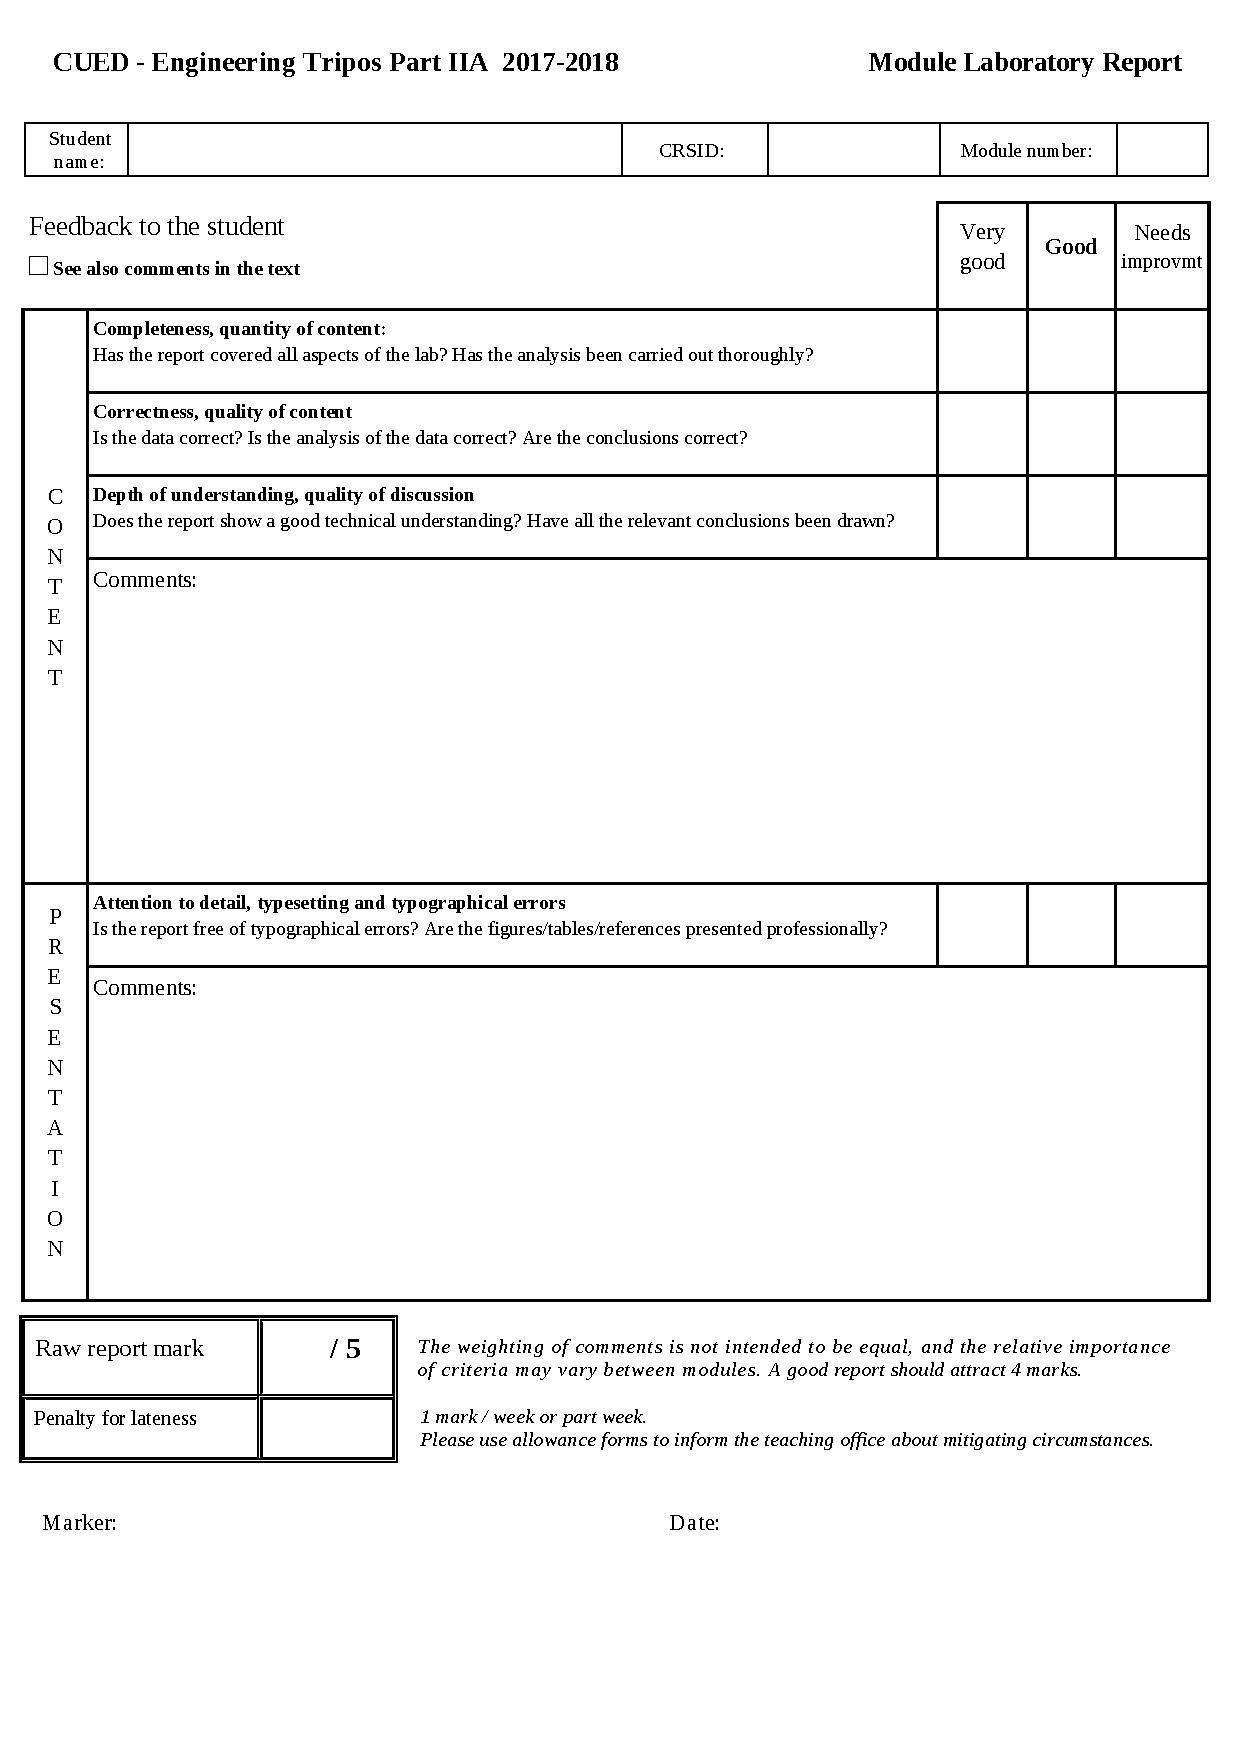
\includepdf[pages={1}]{IIA_Lab_FeedbackSheet_2017.pdf}
\clearpage \mbox{} \pagenumbering{gobble} \clearpage
\pagenumbering{arabic}

%% Lab Report Header %%
\noindent
\rule{17cm}{0.5mm}
\begin{center}
{\bf ENGINEERING TRIPOS PART IIA}
\end{center}
\begin{center}
{\bf 3F8 INFERENCE LAB REPORT}
\end{center}
{\bf Matthew Coates (mc955) \hfill Pembroke College \hfill Lab Date: 16th Feb 2018}
\rule{17cm}{0.5mm}

\section*{Exercise (a)}

\section*{Exercise (b)}

\section*{Exercise (c)}

\section*{Exercise (d)}

\section*{Exercise (e)}

\section*{Exercise (f)}
The final log-likelihood values, averaged over all data points, for the training and test datasets were found to be -0.61 and -0.68 respectively. The confusion matrices for each of the datasets were also found. 
\begin{equation*}
  \text{Training Data} = 
  \begin{bmatrix}
    0.74 & 0.26  \\
    0.28 & 0.72 
  \end{bmatrix}
  \hspace{2cm}
  \text{Test Data} =
  \begin{bmatrix}
    0.66 & 0.34  \\
    0.33 & 0.67 
  \end{bmatrix}
\end{equation*}

\section*{Exercise (g)}

\section*{Exercise (h)}

\subsubsection*{l=0.01}
The final log-likelihood values, averaged over all data points, for the training and test datasets were found to be -0.10 and -0.80 respectively. The confusion matrices for each of the datasets were also found. 
\begin{equation*}
  \text{Training Data} = 
  \begin{bmatrix}
    1.00 & 0.00  \\
    0.00 & 1.00 
  \end{bmatrix}
  \hspace{2cm}
  \text{Test Data} =
  \begin{bmatrix}
    0.52 & 0.48  \\
    0.13 & 0.87 
  \end{bmatrix}
\end{equation*}

\subsubsection*{l=0.1}
The final log-likelihood values, averaged over all data points, for the training and test datasets were found to be -0.09 and -0.39 respectively. The confusion matrices for each of the datasets were also found. 
\begin{equation*}
  \text{Training Data} = 
  \begin{bmatrix}
    0.95 & 0.05  \\
    0.04 & 0.96 
  \end{bmatrix}
  \hspace{2cm}
  \text{Test Data} =
  \begin{bmatrix}
    0.83 & 0.17  \\
    0.14 & 0.86 
  \end{bmatrix}
\end{equation*}

\subsubsection*{l=1}
The final log-likelihood values, averaged over all data points, for the training and test datasets were found to be -0.43 and -0.48 respectively. The confusion matrices for each of the datasets were also found. 
\begin{equation*}
  \text{Training Data} = 
  \begin{bmatrix}
    0.88 & 0.12  \\
    0.08 & 0.92 
  \end{bmatrix}
  \hspace{2cm}
  \text{Test Data} =
  \begin{bmatrix}
    0.90 & 0.10  \\
    0.09 & 0.91 
  \end{bmatrix}
\end{equation*}


\end{document}